\chapter{Implementation}
\label{chap:implementation}
\section{Preparations}
\subsection{Setting up a virtual machine}

For all developments within this thesis a virtual machine was used. This makes it easy to reproduce the environment within the labs at the TKRN group as well as having a portable development solution isolated from the rest of the computer's operating system. As the ROS version called \textit{Kinetic} is widely used within the set-ups around the robot, I will also develop the application using this version. This reduces the risk of incompatibility issues during development. ROS \textit{Kinetic} is available as packages for Ubuntu up to version 16.04\cite{ros:install}, which is why we install this version of Ubuntu within a new virtual machine. Enough virtual hard disk space and memory is assigned to the virtual machine (200GB HDD, 8 GB RAM) as well as 4 processing cores. This set-up should be sufficient for all purposes during this thesis. 

If the virtual machine shall run ROS nodes which have to be accessible by ROS nodes outside the machine itself (i.e. the Android tablet running the control application) the network interface of the virtual machine should be configured as a bridged network connection. This lets the network's DHCP (if present) assign the virtual machine its own IP address reachable from the network. However, this was not possible within the university's network, as Oracle VirtualBox was not able to create a working bridged network adapter using the computer's Wi-Fi connection. During development within the lab another computer directly connected to the university network was used to run \textit{roscore}.

\subsection{Setting up ROS}

\subsubsection{Installing ROS}

Setting up ROS \textit{Kinetic} within a fresh Ubuntu 16.04 installation is fairly simple. First, the ROS apt\footnote{Aptitude is the package management system for Debian-based Linux distributions like Ubuntu}-repository has to be added to the packages sources file and the corresponding key has to be added to the key storage to enable downloading the packages. Once this is done, the package \textit{ros-kinetic-desktop-full} can be installed which will download and install all available packages for ROS \textit{Kinetic}.

The commands to install ROS are denoted in Listing \ref{lst:ros:install}. After these commands have been executed in a terminal window ROS is readily installed.

\begin{minipage}{\linewidth}
	\begin{lstlisting}[caption={Commands for installing ROS\cite{ros:install}},label={lst:ros:install}]
	sudo sh -c 'echo "deb http://packages.ros.org/ros/ubuntu $(lsb_release -sc) main" > /etc/apt/sources.list.d/ros-latest.list'
	sudo apt-key adv --keyserver hkp://ha.pool.sks-keyservers.net:80 --recv-key 421C365BD9FF1F717815A3895523BAEEB01FA116
	sudo apt-get update
	sudo apt-get install ros-kinetic-desktop-full
	\end{lstlisting}
\end{minipage}

ROS is by default installed to \textit{/opt/ros/kinetic/}. To make use of all available command line tools provided by ROS it is important to load the file \textit{/opt/ros/kinetic/setup.bash} into the currently open (bash)-command-prompt. This is either temporarily done by issuing

\begin{lstlisting}[caption={Temporarily loading the ROS environment into bash}]
source /opt/ros/kinetic/setup.bash
\end{lstlisting}

or permanently by adding this line to the file \textit{$\sim$/.bashrc} by executing the following command:

\begin{lstlisting}[caption={Permamently installing the ROS environment into bash}]
echo "source /opt/ros/kinetic/setup.bash" >> ~/.bashrc
source ~/.bashrc
\end{lstlisting}

When this is done, ROS is completely set up on the development machine.

\subsubsection[Setting up catkin]{Setting up a catkin workspace\cite{ros:install:catkin}} 

\textit{Catkin\footnote{\url{http://wiki.ros.org/catkin}}} is a build system and workspace management utility provided with ROS. It supports developers to create, develop and build packages for ROS applications. To create a catkin workspace within the current user's home directory, issue the commands from Listing \ref{lst:ros:catkin} after setting up ROS and sourcing the \textit{setup.bash}-file.

\begin{minipage}{\linewidth}
	\begin{lstlisting}[caption={Setting up a catkin workspace},label=lst:ros:catkin]
mkdir -p ~/catkin_ws/src
cd ~/catkin_ws/
catkin_make

source devel/setup.bash
	\end{lstlisting}
\end{minipage}

ROS and catkin are now fully set up and can be used for further development.

\subsection{Installing Android Studio}

Android Studio is used as IDE during development of this thesis and should be installed according to the official documentation\footnote{\url{https://developer.android.com/studio/install.html}}. It is sensible to add the \textit{bin} directory within Android Studio's installation path to the \textit{PATH} environment variable to make Android Studio accessible by just typing \textit{studio.sh} into a terminal window.

After Android Studio was installed successfully, it is important to select and install the correct Android SDK versions as the project will compile with the Android 7 compiler to work with Android 4. To do so, open The SDK Manager (\textit{Tools > Android > SDK Manager}) and select the SDKs according to Figure \ref{fig:android:sdk}. When this is done, Android Studio is set up to develop and compile the application.

\begin{figure}
	\caption{Needed Android SDKs\label{fig:android:sdk}}
	\begin{center}
		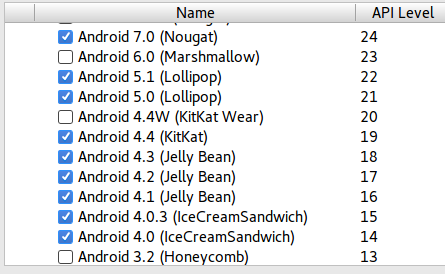
\includegraphics[scale=0.7]{assets/chpt_impl/sdks.PNG}
	\end{center}
\end{figure}

\subsection{Modifying and compiling rosandroid}
\label{impl:compiling_rosandroid}

Since the application developed in this thesis shall work on Android from versions beginning at 4.0.3 we have to modify the rosandroid code on one little detail to make everything work fine. In the created catkin workspace, go to the \textit{src} folder and clone the rosjava and rosandroid repositories there:
\begin{lstlisting}[caption={Cloning the rosandroid and rosjava repositories}]
git clone https://github.com/rosjava/rosjava_core.git
git clone https://github.com/rosjava/android_core.git
git clone https://github.com/rosjava/rosjava_messages.git
\end{lstlisting}

Then line 38 in the file
\begin{lstlisting}[numbers=none]
android_core/android_10/src/org/ros/android/RosActivity.java
\end{lstlisting}

has to be replaced by

\begin{lstlisting}[caption={Change to make to RosActivity.java},firstnumber=38]
public abstract class RosActivity extends android.support.v7.app.AppCompatActivity {
\end{lstlisting}

This gives us the ability to use the already-built features in rosandroid like the automatically displayed activity to connect to a ROS master and built-in node handling even in older Android versions. When changes are made, issue a \textit{catkin\_make} command in the catkin workspace's root directory. \textit{Rosjava} and \textit{rosandroid} will then be built from source and deployed to a \textit{Maven}\footnote{Maven is a dependency and package management system for Java libraries.} repository from where the binaries will be loaded by Android Studio on compile time.

\subsection{Starting the environment}

To start up the development environment with the ROS master, the BioIK service and the \textit{rviz!} simulation of the robot, first the \textit{tams\_cml}\footnote{\url{https://gogs.crossmodal-learning.org/norman.hendrich/tams_cml}} and \textit{bio\_ik\_service}\footnote{\url{https://gogs.crossmodal-learning.org/philipp.ruppel/bio_ik_service}} packages has to be cloned into the catkin workspace, as well as the \textit{tams\_multitouch} package, which has to be copied into the workspace. After \textit{catkin\_make} was executed successfully, the programs are ready to be started. The following commands have to be entered in this order, but within different terminal windows:
\begin{lstlisting}[caption={Commands to start up the development environment}]
roscore
roslaunch tams_multitouch demo.launch
roslaunch tams_f329 4_moveit.launch
rosrun bio_ik_service bio_ik_service
\end{lstlisting}

If interaction with the robot hardware is wanted, the corresponding programs and nodes have to be started according to the file \textit{tam\_cms/tams\_f329/README.txt} within the catkin workspace.

\section{User Interface}
\label{sec:impl:ui}

The user interface of the application was developed according to the considerations made in chapter \ref{chap:concepts}. Additionally it turned out during development, that a basic tele-operation screen for the robot arm would be useful, that enables the user to bring the arm into a defined home position as well as doing simple step-wise manipulation to the robotic arm by moving the desired position of the hand palm by single small steps per button-press. The screen's layout and functionality is described in Section \ref{sec:impl:armteleop}.

The safety interlock button on all screens is immplemented using a \textit{FloatingActionButton}, a predefined conttrol by Android which is designed to float in one corner of the screen above the rest of the screen's contents. To have the \textit{FloatingActionButton} work in the expected way, all screen contents have to be embedded into a \textit{CoordinatorLayout} container. The icon of the button has a \textit{Play} symbol in idle state, in activated state is shows a \textit{Pause} symbol until the button is released. The code to make the interlock button is described in Listing \ref{lst:impl:interlock}. It has to be inserted into the overridden \textit{onStart()} method in every Fragment of the application, in which the functionality shall exist - i.e. every page with controls for the robot.

\begin{lstlisting}[caption={Code for the interlock button}, label=lst:impl:interlock]
@Override
public void onStart() {
	super.onStart();
	
	final FloatingActionButton lockButton = ((FloatingActionButton)getView().findViewById(R.id.lockButton));

	lockButton.setOnTouchListener(new View.OnTouchListener() {
		boolean locked = true;
		
		@Override
		public boolean onTouch(View view, MotionEvent motionEvent) {
			switch(motionEvent.getAction())
			{
				case MotionEvent.ACTION_DOWN:
                        // Code to unlock robot operations
						lockButton.setBackgroundTintList(ColorStateList.valueOf(getResources().getColor(R.color.posOk)));
						lockButton.setImageResource(android.R.drawable.ic_media_pause);
				break;
				
				case MotionEvent.ACTION_UP:
					// Code to lock robot operations
					lockButton.setBackgroundTintList(ColorStateList.valueOf(getResources().getColor(R.color.posNOk)));
					lockButton.setImageResource(android.R.drawable.ic_media_play);
				break;
			}			
			return true;
		}
	});
	
	// ... more code for onStart()
}
\end{lstlisting}

\subsection{Synergy Pages}

\begin{figure}
	\caption{The synergy control screen\label{fig:ui:syn}}
	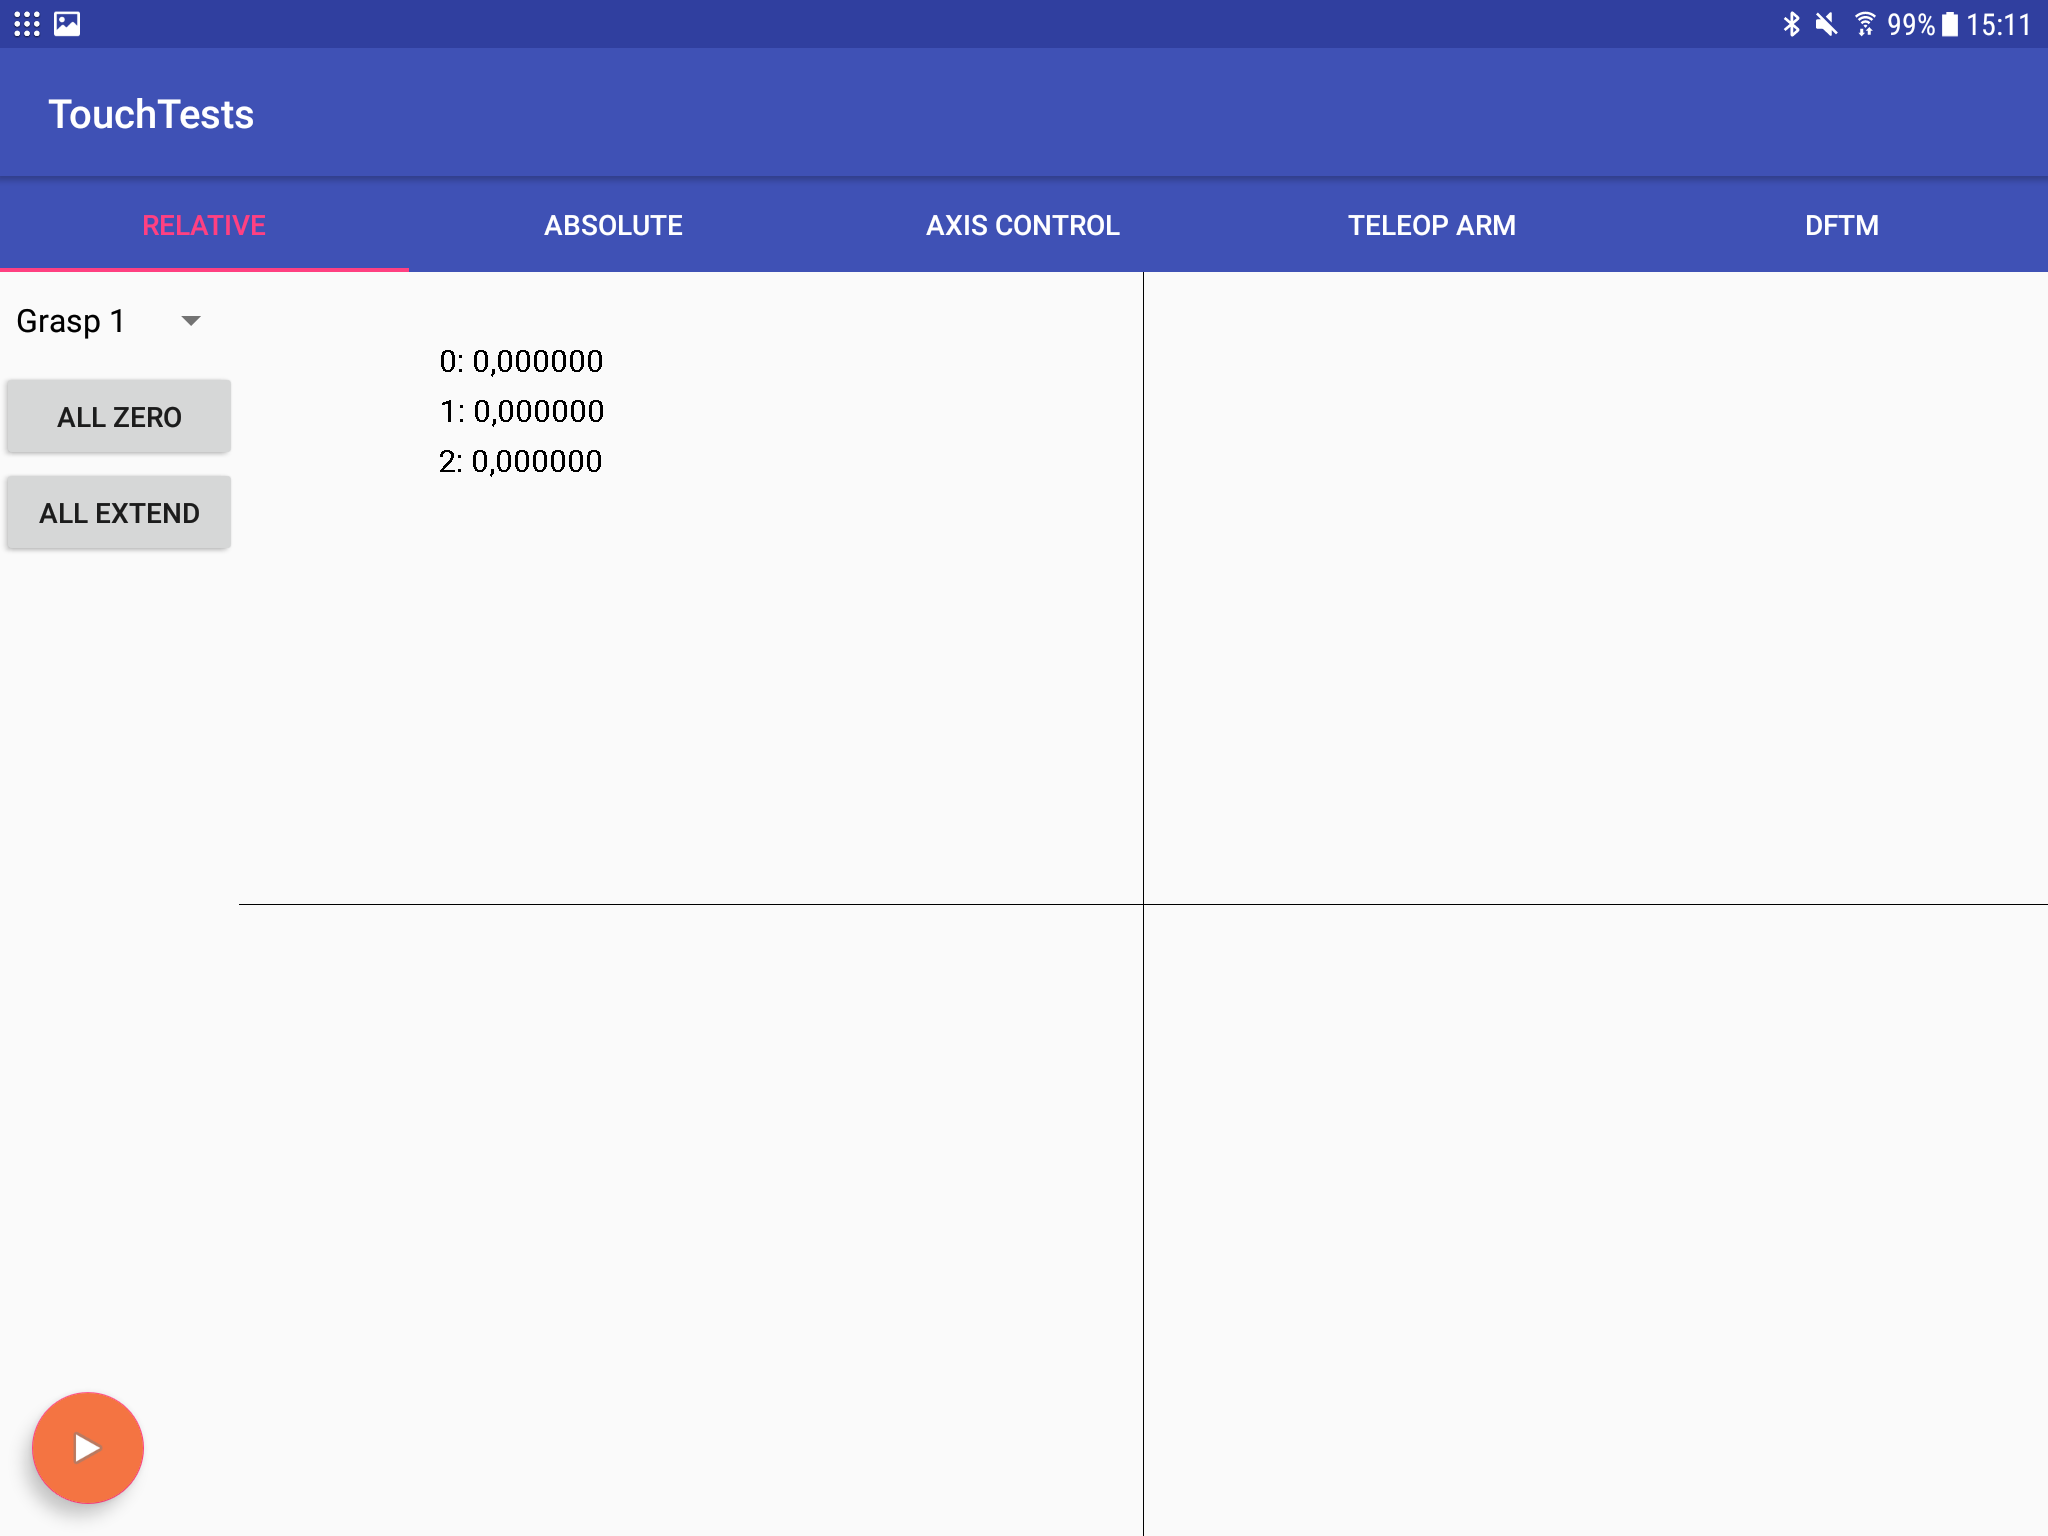
\includegraphics[width=\linewidth]{assets/chpt_impl/syn_blank}
\end{figure}

\begin{figure}
	\caption{display of a two-pointer and a three-pointer gesture on the synergy screen\label{fig:ui:syngest}}
	
	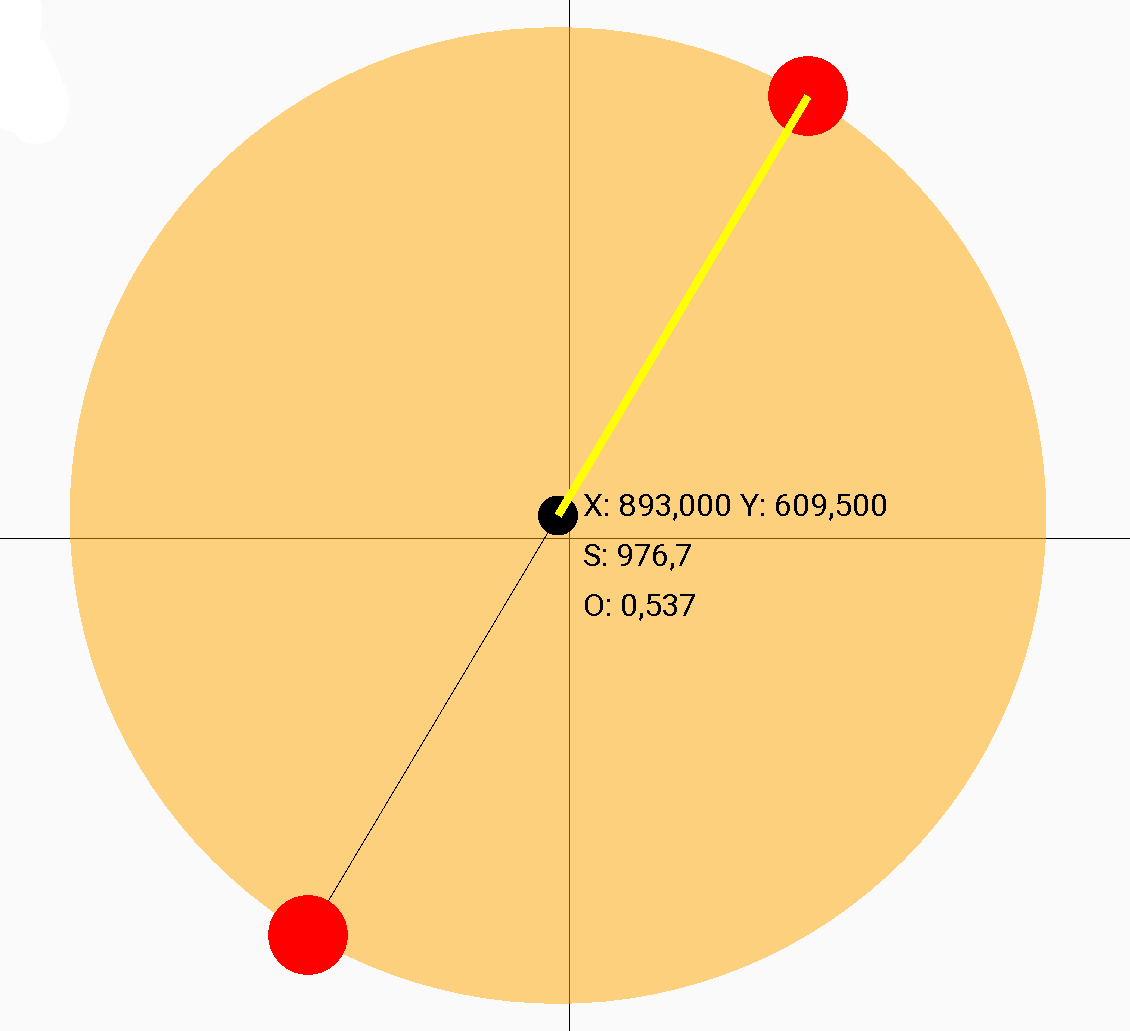
\includegraphics[width=0.5\linewidth]{assets/chpt_impl/syn_2touch}
	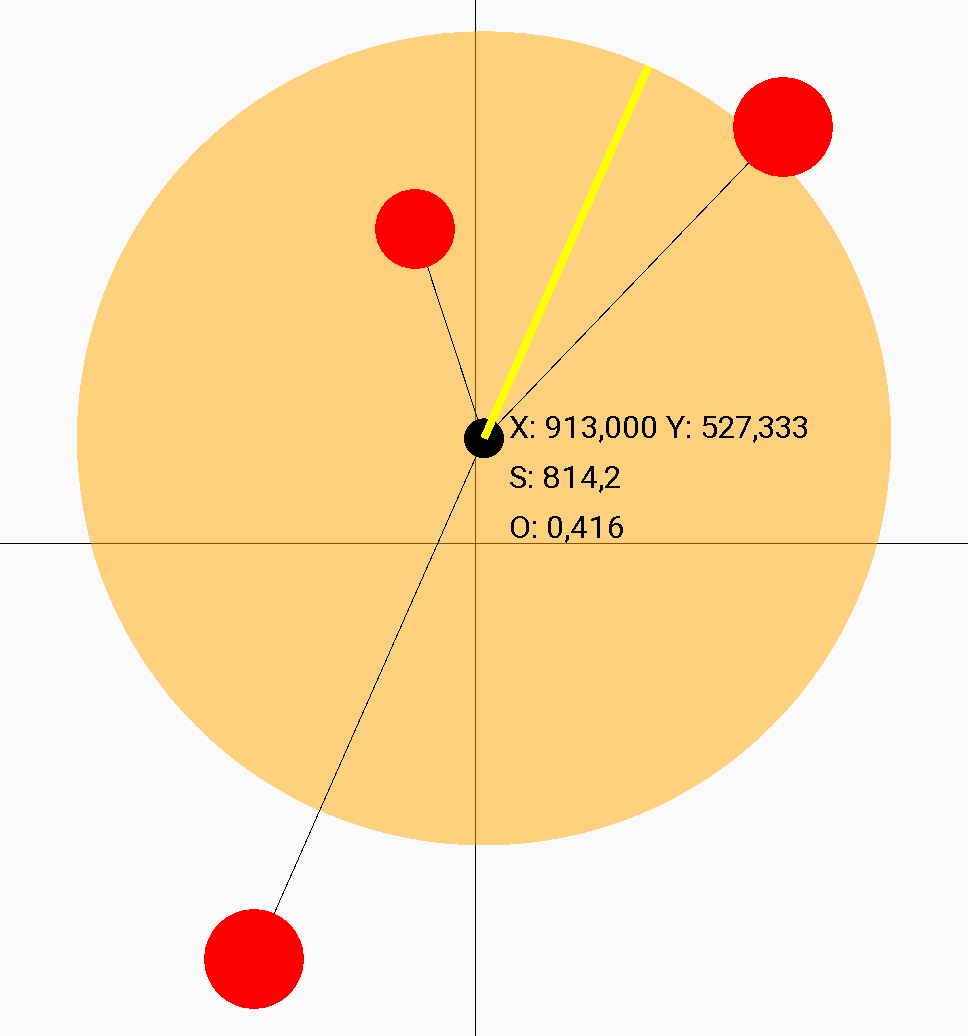
\includegraphics[width=0.5\linewidth]{assets/chpt_impl/syn_3touch}
\end{figure}

The synergy pages are implemented as a mostly blank white page, with a small drop-down control on the left to select the synergy that shall be controlled, as well as a two buttons to set all amplitudes to a known state (i.e. either all zero or all 50). The values of all three controllable amplitudes are displayed in the upper left corner of the control area. The screens for absolute and relative control look the same, which mode is active can be seen in the upper bar with the tab controls. Two lines determine the middle of the control area, which is important for the absolute approach, as the absolute placement of a gesture is important. Figure \ref{fig:ui:syn} gives an impression of how the screen looks on the tablet computer.

Figure \ref{fig:ui:syngest} shows how a two-pointer and a three-pointer gesture is displayed on the synergy pages. While each pointer is marked by a red circle, the center (i.e. the position) of a gesture is displayed as a small black circle, with all pointers being connected to the center by a black line. The orange circle gives an impression of the calculated size of a gesture while the yellow line within the orange circle points in the direction of the orientation which was calculated for a gesture. The calculated values are also displayed in clear text next to the center of a gesture. This is done mainly for debugging purpose, but may also give an interesting insight into the state of a gesture, for example for training purposes. Note that the orientation is not given in degrees, but in radians.

\subsection{Axis Control Page}

\subsection{Direct Fingertip Mapping Page}

\subsection{Arm Tele-Operation Page}
\label{sec:impl:armteleop}

\section{ROS integration}

Thanks to \textit{rosandroid} it is easy to integrate ROS into an Android application. When the libraries are included in the project the main thing to change is that the main activity has to inherit from \textit{RosActivity} instead of the plain Android \textit{Activity} class.

\begin{lstlisting}[caption={Changes to MainActivity}, escapechar=&]
public class MainActivity &\textbf{extends RosActivity}& {
	//...
}
\end{lstlisting}

\begin{wrapfigure}[13]{R}{0.55\linewidth}
\caption{\label{fig:impl:masterchooser}The rosandroid master chooser activity}
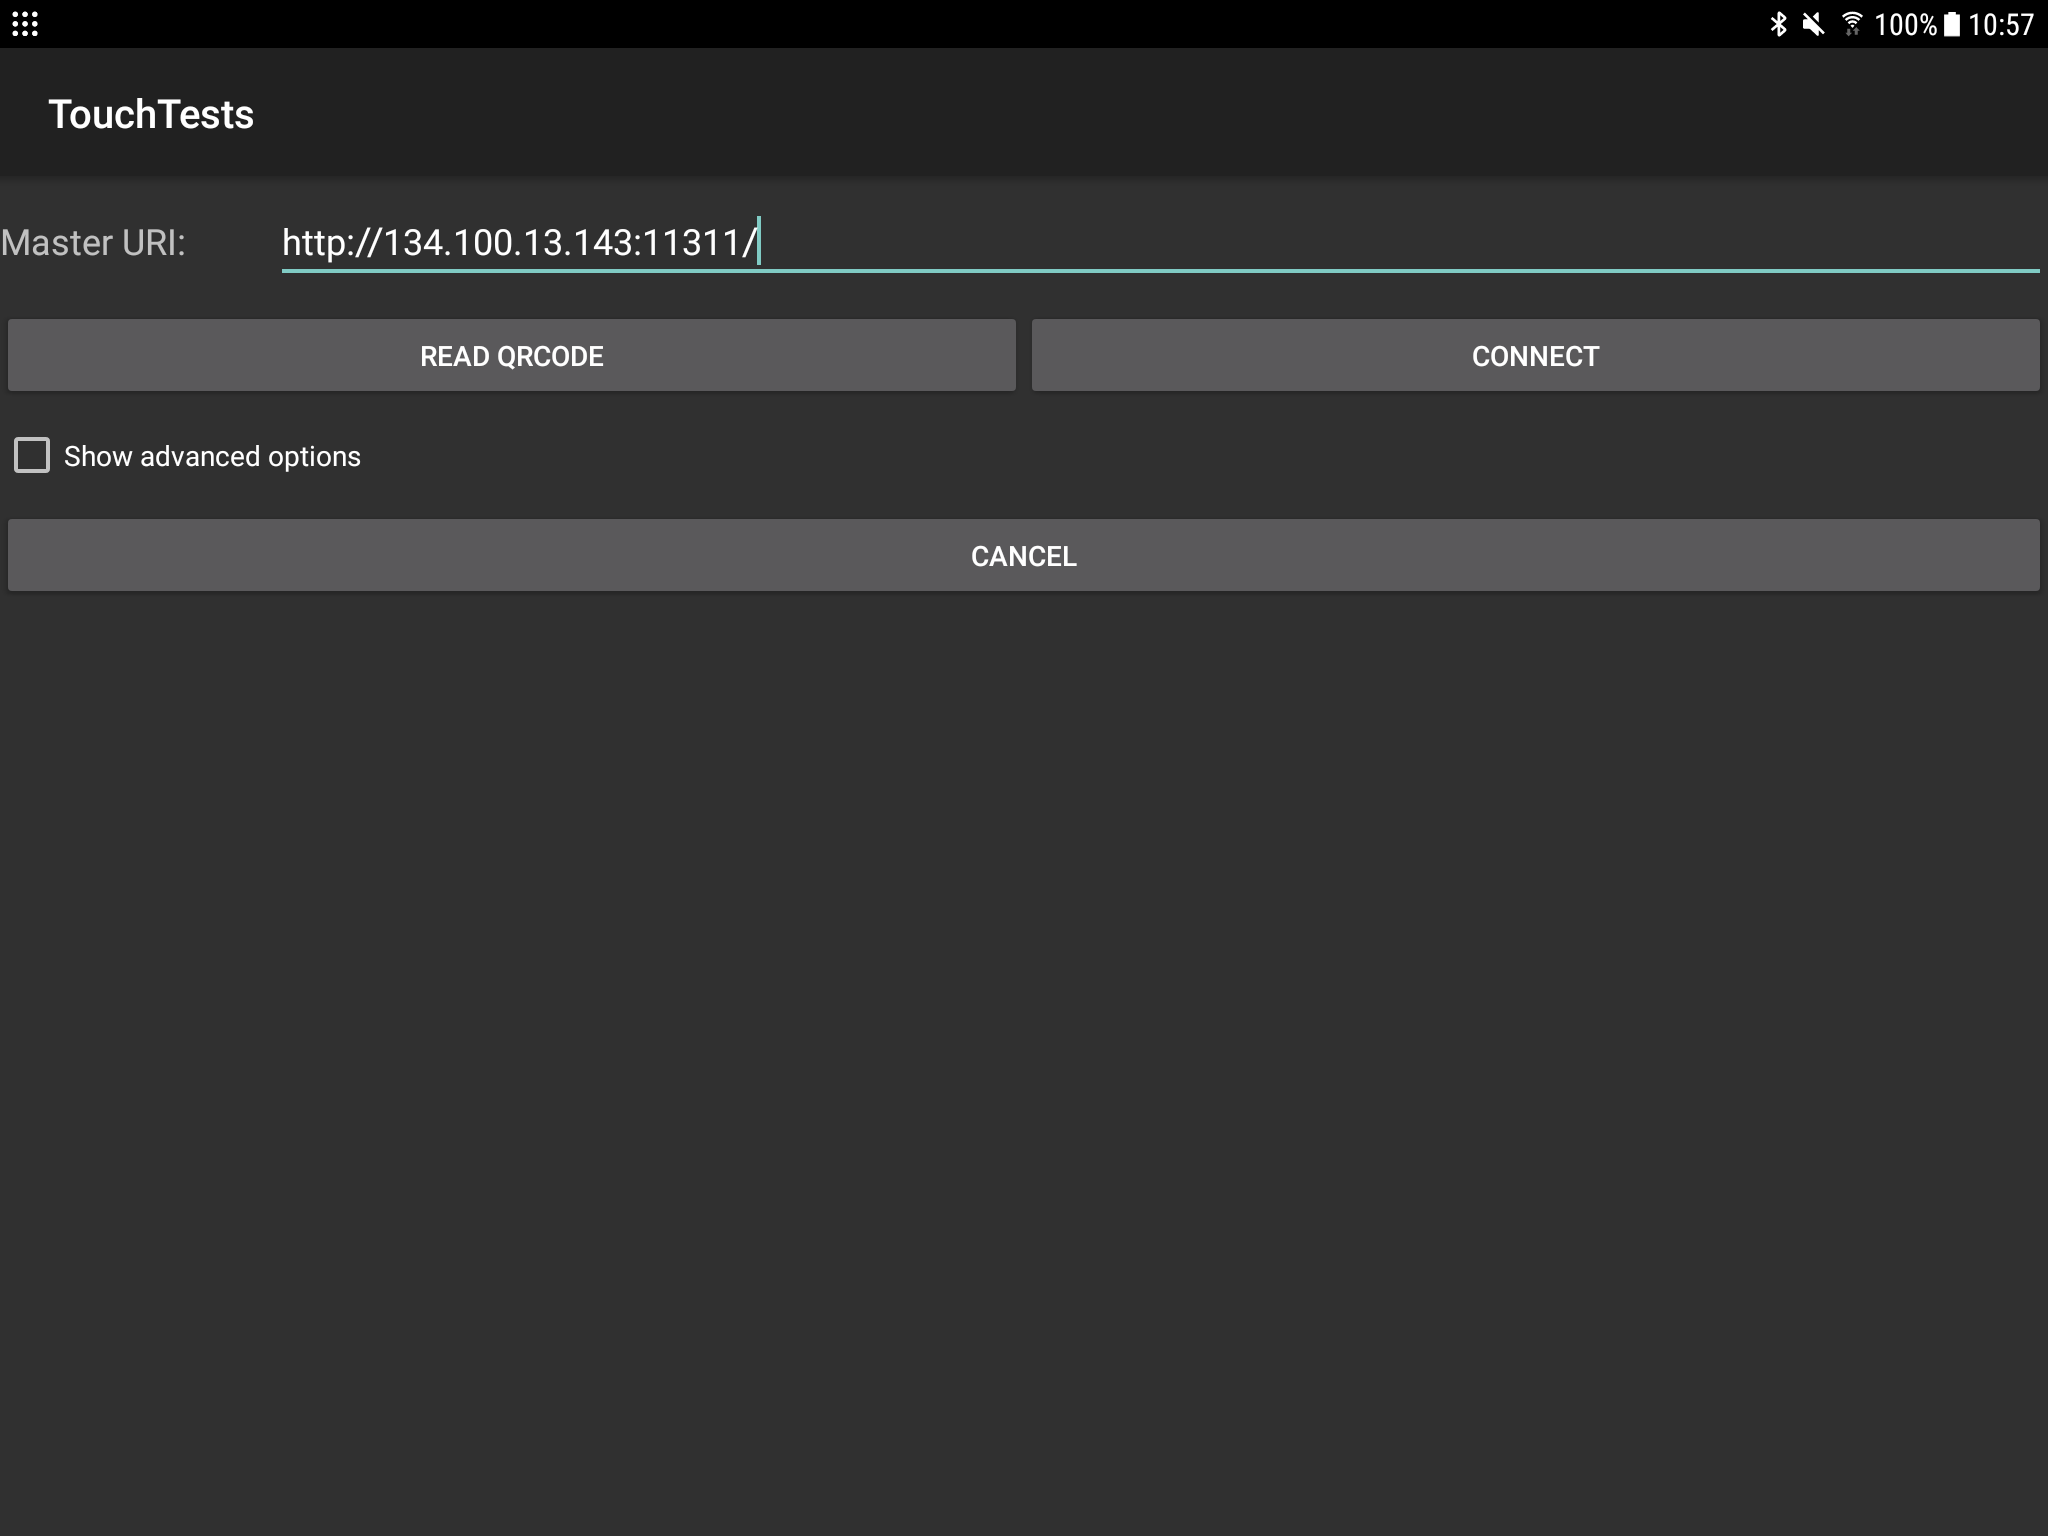
\includegraphics[width=\linewidth]{assets/chpt_impl/masterchooser}	
\end{wrapfigure}

After this change was made, the \textit{RosActivity} implementation takes care about multiple things, beginning with showing a \textit{master chooser}  activity, in which the user can connect to a ROS master node, to handling all connection lifetime events of ROS parts. The \textit{master chooser} activity (see Figure \ref{fig:impl:masterchooser}) lets the user connect to an existing ROS master node. Additionally, it gives the Android application the opportunity to create a dedicated master node on the device itself. As this could affect the overall performance of the application and a lot of functionality has to be run on a more powerful machine, the ROS master is started on a dedicated computer and the Android application connects to this existing master node.

\textit{RosActivity} is an abstract class. To implement it, the \textit{init()} method has to be overriden by inheriting classes. This method is called once the connection to the ROS master node was established and custom nodes can be initialized and connected. All other initialization steps regarding the implemented ROS nodes should also be done here. As shown in Listing \ref{lst:impl:rosconn}\footnote{Information on how to initialize ROS applications was taken from an official rosandroid example found at \url{https://github.com/rosjava/android_core/blob/kinetic/android_tutorial_pubsub/src/org/ros/android/android_tutorial_pubsub/MainActivity.java}}, first an instance of the \textit{C5LwrNode} is created and then assigned to all instances that consume functionality of it (\textit{AxisManager}, \textit{CartesianArmManager}, \textit{DfmtProxy}). After all this is done, the node is registered with the ROS master node. Details on the initialization of the \textit{C5LwrNode} node can be found below in this section. In theory, multiple nodes can be started and registered with the master within one application.

\begin{lstlisting}[caption={Initialization of the ROS connection}, label={lst:impl:rosconn}]
@Override
protected void init(NodeMainExecutor nodeMainExecutor) {
	axisManager = AxisManager.getInstance();
	
	node = new C5LwrNode("/joint_states", "/hand/joint_goals", "/lwr/jointPositionGoal");
	node.addJointDataListener(axisManager);
	
	axisManager.setRobotNode(node);
	CartesianArmManager.getInstance().setNode(node);
	DftmProxy.getInstance().setNode(node);

	NodeConfiguration cfg = NodeConfiguration.newPublic(getRosHostname(), getMasterUri());
	nodeMainExecutor.execute(node, cfg);
}
\end{lstlisting}

\subsection{The C5LwrNode class}

The class \textit{C5LwrNode} inherits from \textit{AbstractNodeMain}, which already offers the very basic lifetime functionality of a ROS node. Some methods have to be implemented by the developer, like \textit{getDefaultNodeName()}, which determines the name of the ROS node as it is registered with the ROS master. In the \textit{onStart()} method, all start-up procedures are implemented, like registering topic subscriptions as well as creating publishers and \textit{service clients}. Within the \textit{onShutdown()} method, all resources created before (subscribers, publishers, service clients) shall be closed and deleted to ensure a clean de-registration from the ROS master and a clean shut-down of the application. The start-up code for the ROS node can be seen in Listing \ref{lst:impl:c5lwrnode}.

\begin{lstlisting}[caption={Startup of the C5LwrNode}, label=lst:impl:c5lwrnode]
@Override
public GraphName getDefaultNodeName() {
	return GraphName.of("ba_android/c5lwrnode");
}

@Override
public void onStart(ConnectedNode connectedNode) {
	cNode = connectedNode;
	handJointStatePub = connectedNode.newPublisher(handPublishTopic, JointState._TYPE);
	armJointStatePub = connectedNode.newPublisher(armPublishTopic, RMLPositionInputParameters._TYPE);

	jointStateSubsc = connectedNode.newSubscriber(subscribeTopic, JointState._TYPE);
	jointStateSubsc.addMessageListener(/* ... */);

	try {
		ikService = connectedNode.newServiceClient("/bio_ik/get_bio_ik", bio_ik_msgs.GetIK._TYPE);
	} catch (ServiceNotFoundException e) {
		ikService = null;
		e.printStackTrace();
	}
}
\end{lstlisting}

The methods that are used to offer the functionality of the \textit{C5LwrNode} are denoted in Listing \ref{lst:impl:c5lwrik}. Because arm and hand joints have to be published to different topics, the \textit{handleJointData()} method calls either \textit{publishHand()} oder \textit{publishArm()}, depending on the parameter \textit{jointType} which is passed by the caller indicating the type of the joint data given. The two methods to request IK solutions from the BioIK service are relatively similar, as both initialize the request with the current robot state passed as a parameter and add a \textit{MinimumDisplacementGoal} to hint the IK solver that a solution is desirable where the least possible movement in all axes is done. The number of attempts is set to $1$, the time-out to find a solution is set to $10ms$ for the palm position and $500ms$ for the fingertip positions. The main difference is that, while for the palm only one \textit{PoseGoal} is added, containing the desired pose of the palm constructed by the x, y, z position and \textit{Quaternion} rotation as passed by the caller, in the method to get a solution for multiple fingertips one \textit{PositionGoal} is added for each fingertip as well as an \textit{OrientationGoal} to have the palm of the robotic hand always point in the same direction. In \textit{GetIKJointsFingertips()}, the \textit{fingertips} parameter contains a map with the link names (e.g. \textit{fftip}, \textit{thtip}...) as key values and the desired 3-dimensional position of the link.

\begin{lstlisting}[caption={C5LwrNode interface},label=lst:impl:c5lwrik]
public class C5LwrNode extends org.ros.node.AbstractNodeMain implements RobotJointDataReceiver {
	private void publishHand(HashMap<String, Double> data);
	private void publishArm(HashMap<String, Double> data);
	
	@Override
	public void handleJointData(int jointType, HashMap<String, Double> data);
	
	public void GetIkJointsPalm(Map<String, Double> currentState, 
		String[] lockedAxes, 
		double x, double y, double z, 
		double rotx, double roty, double rotz, double rotw,
		ServiceResponseListener<GetIKResponse> hdl);
	
	public void GetIKJointsFingertips(Map<String, Double> currentState,
		Map<String, PointInSpace> fingertips, 
		ServiceResponseListener<GetIKResponse> hdl);
}

\end{lstlisting}

\section{The AxisManager}

The most important and most central functionality of the overall application is offered by the \textit{AxisManager} class. It is responsible for holding the current joint angles for all joints in memory, as well as the current target values along multiple other bits of information about each axis or joint. Joints are more generically called \textit{axis} within the \textit{AxisManager}, so this wording will be adopted in the rest of this section.

\subsection{AxisInformation}

All information about an axis is stored in a \textit{AxisInformationImpl} object. This class implements the \textit{AxisInformation} interface, which is returned when axis information shall be given to callers in a read-only manner. The \textit{AxisInformation} interface is given in Listing \ref{lst:impl:axisinformation}. All the information stored about an axis is accessible here. In particular, this is: 
\begin{itemize}
	\item the identifier of an axis, i.e. a string literal containing the name at which the axis or joint is known to the ROS nodes.
	\item the maximum speed the axis may move at.
	\item the target value to which the axis shall be currently moved.
	\item the value representing the axis' current position.
	\item the value representing the axis' \textit{current target value} (see Section \ref{sec:impl:axismovements} for details).
	\item the minimum and maximum values the axis may have as position value.
	\item flags indicating whether the axis is enabled and moving.
	\item an integer representing the type of an axis. Allowed types are \textit{JointType.ARM} and \textit{JointType.HAND}.
\end{itemize}

\begin{lstlisting}[caption={The AxisInformation interface}, label=lst:impl:axisinformation]
public interface AxisInformation {
	String getIdentifier();
	
	double getMaxSpeed();
	double getTargetValue();
	
	double getMaxValue();
	double getMinValue();
	double getCurrentTargetValue();
	double getCurrentValue();
	boolean isMoving();
	double getSpeed();
	boolean isEnabled();
	int getJointType();
}
\end{lstlisting}

All the information is held within the \textit{AxisManager}, referenced by the axis identifier. Manipulation of the data is only done through calls to the \textit{AxisManager}, to give it full control about what happens with all axes. The difference between \textit{AxisInformation} and the concrete implementation \textit{AxisInformationImpl} is, that the implementation has a setter function for every property. All calculations are done within the \textit{AxisManager} itself.

\subsection{AxisManager timer tick}

The \textit{AxisManager} is designed to work fully asynchronous. All information about axes' target values is stored in the according \textit{AxisInformation} object, but only processed from within the main timer event used in \textit{AxisManager}. The timer is set to a frequency of $f_{am} = 10Hz$. This value can easily be changed by altering the static constant field \textit{UPDATE\_FREQ} in the \textit{AxisManager} task. An implementation of a timer is used which gives the ability to schedule an event at a fixed rate. \textit{java.util.Timer} is able to ensure the desired frequency is reached in the long run by slightly alternating the delays between two executions\cite{AndroidTimer2018}. This is important to have axis movements and publishing done at the correct speed and frequency. To use with functionality, the method \textit{scheduleAtFixedRate()} on the timer has to be used. 

All calculations regarding axis movements (Section \ref{sec:impl:axismovements}) are done within the timer tick only. After all calculations have been done the current joint angles are all sent to the \textit{C5LwrNode} to be published over ROS (see Section \ref{sec:impl:aximgrros}).

\subsection{Initialization}

When the application starts or is resumed from a sleeping device (i.e. the screen went off), the \textit{AxisManager} is initialized. This means that it blocks all actions until it has received a specific number of joint states from the \textit{C5LwrNode}. This measure was implemented to prevent the application from sending joint data to a non-existent robot and to initialize the joint data within memory with the current state of the robot. After 20 samples (\textit{JointState}s) have been received, the values are copied into the target values for each axis.
Initializing all joint target values with 0 is obviously not a good choice, as the robot would then go to this position out of any state it is currently in, causing unwanted movements and behaviour. During initialization a modal dialog is shown, blocking all user interaction with the graphical user interface.

\subsection{Axis movements}
\label{sec:impl:axismovements}

The main task of the \textit{AxisManager} is managing movement of all axes in a safe manner. To accomplish this, it restricts the movement for each axis to the maximum speed stored within the \textit{AxisInformation}. Two main modes are available for movement. The first one is by enabling a constant movement of an axis at a specified speed. The second is by setting target values, which the axis will then be moved to at a maximum speed defined on a per-axis basis in the \textit{AxisInformation} object.

\subsubsection{Constant movement}

To set an axis to constant movement at a constant speed, the method
\begin{lstlisting}
public boolean startMoving(String identifier, double speed);
\end{lstlisting}
on \textit{AxisManager} can be called. The parameter \textit{identifier} is filled with the string literal identifying an axis, while \textit{speed} indicates the speed at which the axis shall move. Since only rotational joints are present it the used set-up, the speed (as well as the maximum speed defined in \textit{AxisInformation}) is denoted in $\frac{\text{degrees}}{s}$. The movement speed can be given either positive or negative, depending on the direction the axis shall move in. With this function call, only the information that the axis shall move is stored in \textit{AxisInformation}, actual movement takes place in the timer event, in which the movement speed in clipped to the maximum speed defined for an axis and then divided by the frequency of the timer tick $f_{am}$. In each timer tick event, the position of an axis moving at speed $v$ is altered by $\frac{v}{f_{am}}$. When a constantly moving axis reaches its limit value, the \textit{moving}-flag is not reset, but as the position for an axis is clipped to its maximum and minimum values, no actual movement is done any further. To cancel a constant movement of an axis, simply
\begin{lstlisting}
public boolean stopMoving(String identifier);
\end{lstlisting}
has to be called with the string literal identifying the axis which shall be stopped.

\subsubsection{Setting target values}

The most common use-case in the application is that different parts of the program set values for each axis to be reached. Instead of simply sending the values received by other parts of the program to the robot over ROS, the axis manager implements a safety feature limiting the movement speeds of an axis at a maximum speed. To accomplish this another variable is introduced in \textit{AxisInformation}, the \textit{current target value}. While the \textit{target value} of an axis determines the desired position where the axis shall be at the end, the \textit{current target value} is the value which is actually sent to the robot. The \textit{current target value} is modified in the timer tick.

To change the target value of an axis, \textit{setTargetValue()} has to be called. The signature of the method is
\begin{lstlisting}[caption={Signature of setTargetValue()}, label=lst:impl:settargetval]
public boolean setTargetValue(
	String identifier, 
	double value, 
	boolean force,
	boolean notifyObservers
);
\end{lstlisting}
A call to this method sets the target value $p_t$ of the axis identified by \textit{identifier} to \textit{value}. If \textit{force} is \textit{true}, the smooth movement mechanism described below is overridden and the current target value $p_c$ is directly set to $p_t$ as well. Setting \textit{notifyObservers} to \textit{true} results in the observers of \textit{AxisManager} being notified about the new target value. As the notification often has UI updates as a consequence, it is sensible to notify observers on setting the last value only, not on changing of every value. For convenience, multiple overloads of this method exist, setting either \textit{notifyObservers} to a default of \textit{true}, or \textit{notifyObservers} to \textit{true} and \textit{force} to \textit{false}.

With $p_t$ being the target value as set in \textit{AxisInformation}, $p_c$ the current target value, $v_{max}$ the maximum speed of an axis and $f_{am}$ the frequency of the main timer tick in \textit{AxisManager}, the procedure to move an axis within the main timer tick is as follows:

First, $\Delta p$ is calculated, which is the maximum value change within one timer event, thus
\begin{equation*}
\Delta p = \frac{v_{max}}{f_{am}} \, .
\end{equation*}
Second, the \textit{current target value} is updated as follows:
\begin{equation*}
p_{c,new} = \left\{ 
\begin{array}{ll}
p_t & |p_t - p_c| < \Delta p \\
p_c + \Delta p & |p_t - p_c| > \Delta p \land p_t > p_c \\
p_c - \Delta p & |p_t - p_c| > \Delta p \land p_t < p_c
\end{array}
 \right.
\end{equation*}

The calculated value $p_{c,new}$ is then stored into the \textit{AxisInformation} for each axis.

\subsection{Passing axis data to ROS}
\label{sec:impl:aximgrros}

After each execution of the movement processes described in Section \ref{sec:impl:axismovements}, the newly calculated values are published to the ROS nodes controlling the robot arm and hand. As angles for arm joints and hand joints have to be published to different ROS topics, two calls have to be made. The interface \textit{RobotJointDataReceiver}, which is implemented by \textit{C5LwrNode} has a method
\begin{lstlisting}
void handleJointData(int type, HashMap<String, Double> data);
\end{lstlisting}
accepting the joint type as the first parameter. The ROS node implementation will choose the topic to publish the data to by the given type identifier.

At the end of the timer event in \textit{AxisManager}, first all \textit{current target values} for arm joints are taken from the list of \textit{AxisInformation}. The angle values are converted to radians and put into a Map, which has the axis identifier as the key and the angle of the corresponding axis as value. \textit{handleJointData()} is then called with \textit{JointType.ARM} and the created map. The same procedure is then executed for all \textit{AxisInformation}s with the type \textit{JointType.HAND}.

\subsection{Stopping movement and setting all axes to zero}

Two extra functions are implemented in \textit{AxisManager}. The first,
\begin{lstlisting}
public void copyCurrentValuesToTarget();
\end{lstlisting}
takes all values currently stored as \textit{current value} in \textit{AxisInformation} and copies them into the \textit{target value} and \textit{current target value} fields. This mainly takes the current robot state and copies it into the target state, causing all movements to stop. This is especially useful when the robot cannot reach a position defined by the target position. This is for example the case when all joints of the hand shall be set to $0^\circ$, as some joints are not able to completely reach this value. Copying the currently measured value into the target value stops the robot from trying to reach the actual desired value and, by this, prevents the hardware from being damaged by trying to reach a non-reachable position for too long.

The second special method is
\begin{lstlisting}
public boolean setAllZero(boolean force);
\end{lstlisting}
which sets all axis \textit{target values} to 0. If \textit{force} is \textit{true}, the \textit{current target value} is also set to 0. \textbf{Extreme caution has to be used when calling this function!} The robot will move all joints to a position of 0 degrees either immediately (\textit{force} is \textit{true}) or smoothly. The shortest way in joint space from the current state of the robot to $\vec{0}$ may cause damage to the robot or its environment. This function was implemented to bring the robot to a known state using the axis control page. If the corresponding button is pressed, it is called only after the user has stated that he is aware of the possible dangers.

\subsection{Enabling and Disabling}

The \textit{AxisManager} can be enabled or disabled. In the disabled state, all calls to \textit{setTargetValue()} are discarded. Upon disabling the \textit{AxisManager}, all current measured values of all joints are copied to the \textit{current target value}, causing the robot to stop all movements (see Figure \ref{fig:impl:axisonoff}). The function used to enable and disable the \textit{AxisManager} is
\begin{lstlisting}
public void setLocked(boolean locked);
\end{lstlisting}

This function is designed to be called upon touch actions on the safety interlock button on the user interface pages (see Section \ref{sec:ui:layout}).

\begin{figure}
	\caption{\label{fig:impl:axisonoff}Enabling and disabling the AxisManager}
	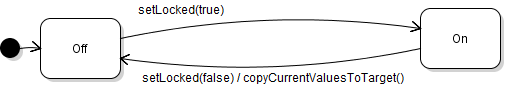
\includegraphics[width=0.75\linewidth]{assets/chpt_impl/sw/AxisManager_onoff}
\end{figure}

\section{Grasp Synergies}
The grasp synergy approach is implemented according to the concepts described in Section \ref{sec:conc:synergy}. The approach are implemented using a gesture page and relative and absolute approach are differentiable by the title of the tabbed page selector, apart from that, the pages look the same.

\subsection{Gesture Parsing}

Gesture parsing is separated into multiple classes. The \textit{GestureParser} class accepts touch events redirected to it by the \textit{GestureView}s on the pages for gesture control. It has a method 
\begin{lstlisting}
public void handleTouchEvent(MotionEvent e);
\end{lstlisting}
which is called from within the \textit{onTouchEvent()} handler of the user interface element. The \textit{GestureParser} is otherwise independent from the user interface element it is invoked by. When a new pointer is encountered, it adds it to a gesture it fits to which is already present on the screen or -- if the pointer is too far away from any existent gesture -- creates a new gesture. If a pointer is removed from the screen, it is also deleted from the gesture it was assigned to. If no pointers are left within the gesture, it is also removed. If an event is received stating a pointer has moved, the pointer location is updated in memory. Upon all of the described actions, the observers of the \textit{GestureParser} are notified. These observers implement the \textit{GestureObserver} interface, which is shown in Listing \ref{lst:impl:gestobs}. It gives the \textit{GestureParser} to notify observers about the addition or removal of a gesture, as well as the case on which a pointer of the gesture has changed its position. 

\begin{lstlisting}[caption={The GestureObserver interface}, label=lst:impl:gestobs]
public interface GestureObserver {
	void onGestureAdd(Gesture g);
	void onGestureRemove(Gesture g);
	void onGestureChanged(Gesture g);
}
\end{lstlisting}

If the pointer count of a gesture changes, the \textit{GestureParser} calls the \textit{onGestureRemove()} method of observers, and then the \textit{onGestureAdd()} method. Both with the same \textit{Gesture} object.

When a gesture is added or its pointer count changes, it is marked as \textit{locked} by the \textit{GestureParser} for the duration of one second. This indicates to dependent classes, that the gesture is new and the data should not yet be used for any control purposes, as the user might still adjust finger positions. This also takes care of the fact that, to add a multi-pointer gesture, the android system calls different events for each pointer subsequently, meaning that to the software it looks as if a one-pointer gesture was added, then a two-pointer gesture and then a three-pointer gesture, if 3 fingers were laid on the touchscreen. By ignoring gesture input for the first second of a new gesture, the user should have put all fingers onto the screen and can then control the application. Having input by an unwanted gesture may cause unexpected behaviour. In the following the functionality of the three main material classes \textit{Location}, \textit{Pointer} and \textit{Gesture} is explained.

\subsubsection{The Location class}

The \textit{Location} class represents a two-dimensional vector within the program. It has two coordinates, $x$ and $y$, which can be accessed by getter methods. It also offers basic functionality to work with vectors, including addition, subtraction, multiplication with scalars and the scalar-product. All functionality is implemented as expected by common sense. When a mathematical operation is performed using two \textit{Location} objects, the result is returned as a new one, as a \textit{Location} is immutable once it is created.

\begin{lstlisting}[caption={The public interface of the Location class}, label=lst:impl:location]
public class Location {
	public Location(float x, float y);
	
	public float getX();
	public float getY();
	
	public Location add(Location loc);
	public Location substract(Location loc);
	public Location multiply(float c);
	public Location divide(float c);
	
	public double scalarProduct(Location loc);
	
	public double getVectorLength();
	public double distanceTo(Location loc);
	public double getAngleTo(Location loc);
	public Location getTurned(double angleRad);
	public boolean isSame(Location l2);
}
\end{lstlisting}

As visible in Listing \ref{lst:impl:location} multiple advanced operations are also available on \textit{Locations}. \textit{getVectorLength()} returns the length of the vector calculated using the Pythagorean theorem. \textit{getDistanceTo()} is implemented very similar, as it basically calculates the length of the differential vector between the \textit{Location} it is invoked on and the passed second \textit{Location}. Although this could be done by one \textit{substract()} operation and then performing \textit{getVectorLength()} on the result the calculation is directly implemented here for performance reasons.

\begin{lstlisting}[caption={Implementation of getVectorLength() and getDistanceTo()},label=lst:impl:location_length]
public double getVectorLength() {
	return Math.sqrt(Math.pow(x, 2) + Math.pow(y, 2));
}

public double distanceTo(Location loc) {
	return (float)Math.sqrt(Math.pow(loc.x - this.x, 2) + Math.pow(loc.y - this.y, 2));
}
\end{lstlisting}

\textit{getAngleTo()} returns the angle between the \textit{Location} it is invoked on and the one passed as a parameter. Please note that this represents the calculation as defined in Equation \ref{eq:conc:orientation} implemented for arbitrary vectors. This means that the output of this method ranges from $-\pi$ to $\pi$, with positive angles meaning a clockwise rotation from the invoked \textit{Location} to the one passed as a parameter. The reader if referred to Listing \ref{lst:impl:angles} for the implementation of \textit{getAngleTo()}. In Line 4 the determinant of the two combined vectors is calculated and the result is multiplied with $-1$ if the determinant is negative. This could've been written shorter, but for better readability this format was chosen.

\begin{lstlisting}[caption={Implementation of getAngleTo()},label=lst:impl:angles]
public double getAngleTo(Location loc) {
	double val = Math.acos(scalarProduct(loc) / (getVectorLength() * loc.getVectorLength()));
	
	if(x * loc.getY() - y * loc.getX() < 0) {
		val *= -1;
	}

	return val;
}
\end{lstlisting}

Lastly, \textit{getTurned()} returns the current \textit{Location} rotated by an angle of \textit{angleRad}. The angle may range from $-\pi$ to $\pi$, with positive angles meaning a clockwise rotation. \textit{isSame()} is a numerical comparison of the two vectors. Note that floating point numbers are compared here, on which equality comparisons are problematic. This function is used to check for exactly the same values, meaning probably the same location objects.

\subsubsection{The Pointer class}

Pointers are the contents of \textit{Gestures}. They contain of a \textit{Location}, representing their coordinates on the touch-screen and an id, which is their touch-pointer-id as assigned by the Android operating system. This class was basically introduced to semantically separate the pointer id from the location. The id is needed to identify a pointer within the motion event raised by the operating system. A method is provided to update the location of a pointer, in which a new \textit{Location} object is created.
\begin{lstlisting}[caption={The Pointer class}]
public class Pointer {
	public Pointer(int id, float x, float y);

	public int getId();

	public Location getLocation();
	public void setLocation(float x, float y);
}
\end{lstlisting}

\subsubsection{The Gesture class}

The \textit{Gesture} class represents a gesture as defined in Section \ref{sec:conc:gestures}. It is basically a set of \textit{Pointer}s with a set of properties. Its public interface is denoted in Listing \ref{lst:impl:gestureclass}.

\begin{lstlisting}[caption={Public interface of the Gesture class},label=lst:impl:gestureclass]
public class Gesture {
	public boolean isLocked();
	public void setLocked(boolean locked);
	
	public void addPointer(Pointer p);
	public void removePointer(Pointer p);
	public int getPointerCount();
	
	public boolean catchesPointer(Pointer p);
	public float getCatchRadius();
	public float getDistanceToCenter(Pointer p);
	
	public Location getCenter();
	public float getSize();
	public double getOrientation();
}
\end{lstlisting}

The first two methods set and query the \textit{locked} state of a gesture, followed by three methods to add and remove pointers, as well as querying the number of currently available pointers in a gesture. Whenever a pointer is added or removed to or from a gesture, the \textit{thumb pointer} is evaluated according to the rules defined in Section \ref{sec:conc:gestures}.
\textit{catchesPointer()} determines whether a new \textit{Pointer} can be added to the gesture. This is done by checking whether the \textit{Pointer}  is within a distance of $2.5$x the size of the gesture around its center. If only one pointer is present in a gesture no size is available. In that case, a size of 1200 is taken as the \textit{catch radius}. \textit{getCenter()}, \textit{getSize()} and \textit{getOrientation()} represent $c(G)$, $s(G)$ and $o(G)$ as defined in section \ref{sec:conc:gestures}.

\subsection{Arm Control}

\subsubsection{The PointInSpace class}

The \textit{PointInSpace} class implements functionality as a vector in three dimensions, offering basic operations like adding other \textit{PointInSpace} instances and multiplying with scalars. It is not as elaborated as the \textit{Location} class, but extending the functionality according to \textit{Location} if needed could easily be done.

\begin{lstlisting}[caption={The public interface of PointInSpace}]
public class PointInSpace {
	public PointInSpace(double x, double y, double z);
	
	public double getX();
	public double getY();
	public double getZ();
	
	public PointInSpace add(PointInSpace pw);
	public PointInSpace multiply(double v);
}

\end{lstlisting}

\subsubsection{The CartesianArmManager class}

The functionality to move the arm (or better: The palm of the robotic hand) in Cartesian space is provided by the \textit{CartesianArmManager}. It accepts positions for the palm and manages the querying of the BioIK service asynchronously in the background. Once it received a result from the IK service it forwards it to the \textit{AxisManager} instance. It holds a list of all joints that shall not be affected by the \textit{CartesianArmManager}, i.e. all joints of the Shadow C5 hand, thus placement of the palm only takes place by moving joints belonging to the Kuka robot arm. It also only updates joints in the \textit{AxisManager} that it shall affect, leaving control to all the other joints to different parts of the software.

\begin{lstlisting}[caption={The public interface of CartesianArmManager}, label=lst:impl:cartarm]
public class CartesianArmManager implements ServiceResponseListener<bio_ik_msgs.GetIKResponse> {
	public static final double Y_MIN = -1.2;
	public static final double Y_MAX = -0.8;
	public static final double X_MIN = -0.2;
	public static final double X_MAX = 0.4;
	public static final double Z_MIN = 1.05;
	public static final double Z_MAX = 1.17;
	
	public static final int MAX_AXIS_CHANGE = 15;
	
	public static CartesianArmManager getInstance();
	
	public void setNode(C5LwrNode node);
	
	
	public boolean goHome();
	public boolean movePalm(PointInSpace offset);
	public boolean movePalmTo(PointInSpace position);
	
	public PointInSpace getPosition();
	
	public void stop();
}
\end{lstlisting}

\begin{wrapfigure}[20]{R}{0.5\linewidth}
	\caption{\label{fig:impl:cartarmstate}State diagram for the CartesianArmManager update loop}
	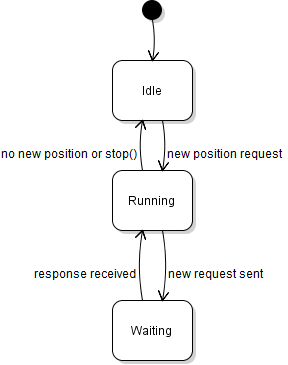
\includegraphics[width=\linewidth]{assets/chpt_impl/sw/CartesianArmManager_loop}
\end{wrapfigure}

Whenever a new target position for the palm is set using \textit{goHome()}, \textit{movePalm()} or \textit{movePalmTo()}, the IK-loop within the \textit{CartesianArmManager} is started. It tries to get solutions from as BioIK service as fast as it can, initiating a new request as soon as one result was received until either no new position was requested or \textit{stop()} was called. Once one of these two cases happen, the loop is stopped and restarted only when a new position is set. Whenever the loop starts a new request, it uses the last set value as target value, values set in between two requests are omitted. Figure \ref{fig:impl:cartarmstate} gives an overview about this process in form of a state diagram.

When a result is returned by the BioIK service it has to go through multiple checks before it is sent to the robot. First, if the \textit{error\_code} field has another value than $0$, the BioIK solver could not find any solution for the queried robot pose, in this case, the \textit{CartesianArmManager} sends the same request to the BioIK service again so it tries to find another solution again. If the \textit{error\_code} field is $0$, the joint angles from the solution are compared to the currently measured state of the robot. When one joint is changed by more than 15 degrees, the solution is rejected as unsafe and a new solution for the same request is queried at the BioIK service. This is done to prevent big movements in joint space, possibly causing unwanted and uncontrollable movements of the robot, potentially causing damage to the robot or its environment. The check for high distances in joint space can be bypassed, which is used when letting the robot go into home position, as this specific position most probably has a bigger distance to the state before than allowed by the check. This means that \textbf{when going to the home position, the user has to watch the robot and has to use caution when using this functionality.} Whenever unwanted movement is observed the user can lift the finger off the safety interlock button to immediately stop any robot movement. As an additional precautionary measure, a hardware emergency switch should be within reach of the operator. When the above checks pass, the joint angled of the arm returned by the BioIK service are written to the \textit{AxisManager} which then sends them to the robot over ROS.

The functionality of the three methods to set new target value is in particular:
\begin{itemize}
	\item \textit{goHome()} sets the target position of the palm to a fixed position which is known to be safely reachable. In this case, it's $p_{home} = \vecthr{0}{y_{min}}{z_{max}}$, which is a position located directly in front of the robot at the border of the table.
	\item \textit{movePalm()} moves the current target position of the palm by \textit{offset} (by adding it to the position returned by \textit{getPosition()}).
	\item \textit{movePalmTo()} overwrites the target position by \textit{position}.
\end{itemize}



\subsection{Absolute control}

\subsection{Relative control}

\section{Direct Finger Positioning}

\section{Performance}

\subsection{Application}

\subsection{BioIK Service}